\model{Using IDLE}

``IDLE is Python's Integrated Development and Learning Environment.
It has two main window types: the Shell window and the Editor window.
It is possible to have multiple editor windows simultaneously.''
(Source:~\url{https://docs.python.org/2/library/idle.html})

\bigskip
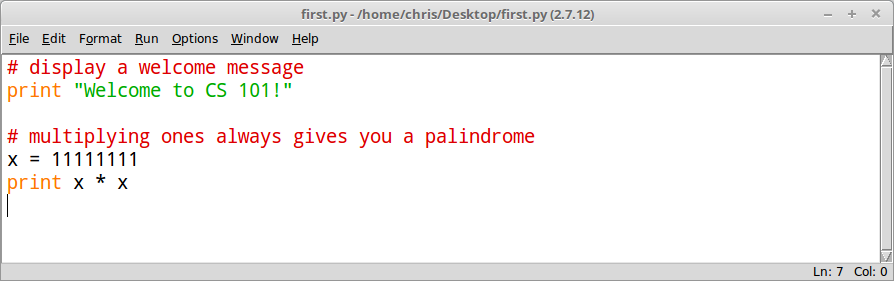
\includegraphics[width=0.8\linewidth]{idle-editor.png}

\bigskip
\hfill 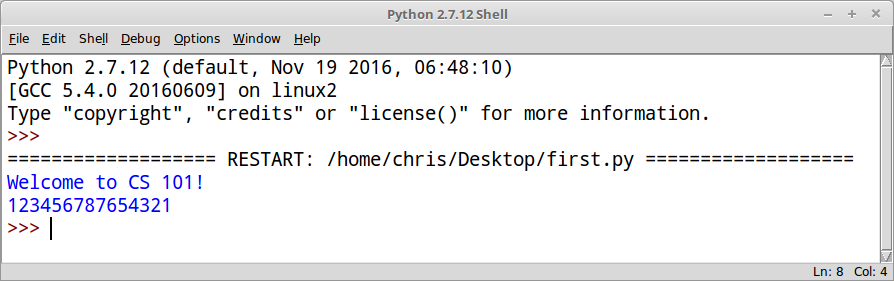
\includegraphics[width=0.8\linewidth]{idle-shell.png}


\quest{15 min}


\Q Which of the two screenshots in \ref{idle.tex} is the Shell window?
Which is the Editor window?

\begin{answer}
The top window is the editor, and the bottom window is the shell.
You can tell based on the window titles.
\end{answer}


\Q Explain the terms ``Editor'' and ``Shell'' based on what you learned previously in the course.

\begin{answer}
An editor is a simple program for writing plain text files.
A shell (or terminal) is an interface for running commands.
\end{answer}


\Q What is the name of the file in the editor? What directory is it saved in?

\begin{answer}
The name is first.py, and the directory is Desktop.
\end{answer}


\Q Explain the Python code in the editor window. What does each line do?

\begin{answer}[5em]
The first line is a comment, the second line displays a message, the third line is blank, the fourth line is another comment, the fifth line creates a variable named x, and the sixth line displays the value of x squared.
\end{answer}


\Q What is the output of the program? Where should you look for output?

\begin{answer}[5em]
The output is in the shell window (in blue): \\[2pt]
\hspace*{2em} Welcome to CS 101! \\
\hspace*{2em} 123456787654321
\end{answer}


\Q Predict the output of each line below. Then type each line into the Shell window (one at a time) and check your answers.

\begin{enumerate}
\item \pyth{print 2 * 5} \ans{10}
\item \label{add} \pyth{print 2 + 5} \ans{7}
\item \label{str} \pyth{print "2 + 5"} \ans{2 + 5 ~ (without quotes)}
\item \label{err} \pyth{print CS rocks!} \ans{SyntaxError: invalid syntax}
\item \pyth{print 2 # 5} \ans{2 ~ (because \pyth{#} makes a comment)}
\end{enumerate}

\Q Explain the difference between \ref{add} and \ref{str} in the last question. Why are the results different?

\begin{answer}
\pyth{2 + 5} computes the number 7, whereas \str{2 + 5} is literal text.
\end{answer}


\Q What is wrong with the code in \ref{err}? Explain the error message. How do you fix the error?

\begin{answer}
It's interpreting the code \pyth{CS rocks!} as an arithmetic expression, but it's not valid (e.g, there's no operator). Syntax error means the code is not correctly structured. Add quote marks around \str{CS rocks!} to fix that line.
\end{answer}
